\documentclass[12pt]{article}
\usepackage[a4paper,margin=1in]{geometry}
\usepackage[utf8]{inputenc}
\usepackage[english]{babel}
\usepackage{graphicx}
\usepackage{csquotes}
\usepackage{setspace}
\usepackage{biblatex}
\usepackage{hyperref}

\graphicspath{{./}}
\addbibresource{bibliography.bib}

\title{A Machine Learning Approach to Building a Chess Engine}
\author{Daniel Cloutier \and Sagar Patel}
\date{\today}
\doublespacing

\begin{document}
    \begin{singlespace}
        \maketitle 
    \end{singlespace}

    \tableofcontents

    \clearpage

    \begin{abstract}
        In the current era, high volumes of data are being collected at an incredible velocity. Much of this data is embedded with valuable knowledge. \cite{main} One example of the types of data that is collected is chess data. In fact, \href{https://lichess.org/}{lichess.org}, one of many websites where chess can be played online against opponents from around the world, contains a data dump of over one and a half billion games, seventy eight million of them being played in the month of November 2020 alone \cite{lichessdb}. We intend to present an automatic learning method for chess, utilizing deep neural networks. We created our deep neural network using a combination of both unsupervised and supervised training. Employing unsupervised training, our engine pre-trains to identify and extract high-level features that exist in a dataset of chess board positions. The supervised training compares two chess positions and evaluates the board which is more favourable, from the white player's perspective. Therefore, we create a deep neural network that can understand chess without incorporating the rules of the game and using no prior manually extracted features. Instead, the system is trained from end to end on a large dataset of chess positions. The resulting deep neural network should allow for simulations that extend the possibilities of chess strategies, highly valuable to chess players at all levels.
    \end{abstract}
        
    \section{Introduction}
    The game of chess is a very popular board game and has become a well liked study for computer enthusiasts, especially in the domain of Artificial Intelligence, from the creation of Deep Blue in 1996 which defeated the world chess champion at the time, Garry Kasparov, up to modern data analysis techniques being tested on chess games as a show for it is possible uses \cite{maiachess}\cite{piece_values}\cite{alphazero}. Chess has become a good starting point for both more advanced software developers attempting to test something innovative or for newcomers trying to increase their knowledge. 

    One of the many reasons for the game's popularity is that chess data is collected at an incredibly high volume and velocity. Not only this, but the data collected is often readily available to the public. Databases such as \href{https://database.chessbase.com/}{chessbase} and \href{https://database.lichess.org/}{lichess} contain thousands, if not millions of games in a standardized notation format for chess called Portable Game Notation. This makes the game of chess a perfect starting point for new tools in Data Science to be tested.

    Another of the many domains of study that has been recently using chess as a means of improving itself is that of Machine Learning. Namely, with the advent of algorithms such as AlphaZero \cite{alphazero}, some new ideas have risen in an attempt to create algorithms that not only play chess better than humans, but even some that try and mimic human play \cite{maiachess}.

    Keeping all of this in mind, we wanted to take advantage of the very large amount of data stored by \href{https://lichess.org/}{lichess} in order to implement and perhaps try and reinvent some already existing ideas using this data that, as far as we could tell, has not been used much in recently published material.
    
    \section{Review of Research and Ideas}

    \subsection{Chess Game Categorization}

    A possibility for using this data is to attempt to categorize chess data into different groups based on some sort of requirements that we could find. For example, perhaps we could group games based on similar openings, similar player ratings or perhaps try to find some different parameters to use to categorize them. One example comes by defining a distance between two games.

    One such way is defined as follows. Defining a nine dimensional space, consisting of the x-y location of a piece before it has been moved as well as after, a weight for the piece before it was moved as well as after (because of piece promotion) as well as the piece that was captured, as well as x-y locations for the piece that was captured. From here you can compare moves between games and calculate the distance between them to figure out what games are similar and what games are outliers \cite{main}. This information could be easily stored although incredibly voluminous. Every move of the game would be stored as nine seperate values. Figures 1 and 2 show how storing this information could look.

    
        \begin{figure}[ht]
            \centering
            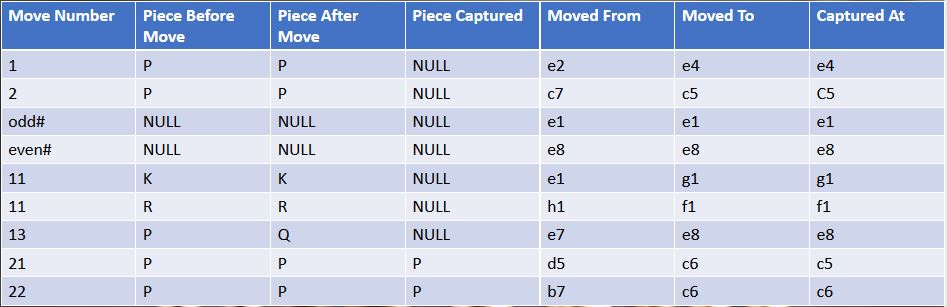
\includegraphics[width=0.9\textwidth]{9dboard.jpg}
            \caption{How storing the above information would look like}
        \end{figure}
        \begin{figure}[ht]
            \centering
            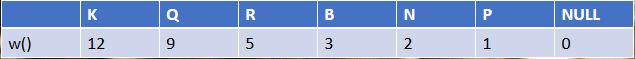
\includegraphics[width=0.7\textwidth]{sampleweights.jpg}
            \caption{Sample weight values for pieces}
        \end{figure}

    From here on we can define the distance between two moves as a euclidean distance between two moves defined by this nine dimensional space. To extend this further, we can define the distance between two whole games as a sum of the distance between corresponding moves. This would be defined as 

    \begin{equation}
        dist(F, G) = \sum^{M}_{i=1} dist(F[i], G[i])
    \end{equation}

    where F[i] is the $i$-th move of game F, G[i] being the $i$-th move of game G and M is the greater of the maximum number of moves from either game \cite{main}. Appending a NULL move as necessary.

    This kind of categorization could be very useful for new and old players alike. To be able to choose a game and immediately be given results for similar games is a very powerful learning tool. There are often \href{https://www.chessstrategyonline.com/content/tutorials/basic-checkmates-smothered-mate}{patterns} that can emerge from chess positions which can likely be spotted by thorough study of similar positions or games. Also, for an advanced player, studying games that lie outside of the norm can be a good way to surprise unexpecting opponents with new ideas.

    The above is in fact a type of unsupervised artificial intelligence. But what we can also do by using data mining techniques is create a supervised pattern matching algorithm to classify similar positions \cite{main}. Once again, this idea can help categorize games into buckets which can then be looked at if there are certain themes that you know of which appear in a certain group. Seeing other similar games could grant some insight into those types of positions, whether you want to learn the basics of them or want some fresh ideas to improve your play.

    \subsection{Predicting Game Results}

    Following from the previous idea, we could try to use the data in an attempt to predict the result of a game. The lichess database contains a lot of information which others might not. Based on our research, most uses of chess data was limited almost exclusively to Grandmaster games, in a specific time control. Lichess contains players of all levels, games are played in all sorts of time controls including fast one minute "bullet" games, all the way up to thirty minute slow games \cite{lichessdb}. Using all of this information, along with what was defined previously and the fact that we know the result of every game in the database, we could try and define some way to predict whether a current game of chess, given the player ratings, other similar games, time control and so on, is going to be a win for white, black or a draw.

    For example, say we could plot all games according to their similarity distance as defined above \cite{main}. However, if we were to include things like player rating, opening used, time control and so on, we could plot games on multiple dimensions. From here, by looking at games similar to an input game and looking at their results, we could make an attempt at predicting what the result of that game will be in its current state.

    There's even more than we can do still. The lichess database starting April 2017 also includes the exact clock times on every single move played. Keeping this in mind means we can improve the above idea further. Some of these could be including the current amount of time each player has, trying to improve the way we define how similar two games are or even by defining a function for determining whether a board position is winning or losing from the white player's perspective assuming best play, not unlike what modern chess computers do \cite{stockfish}. 

    Using the above information we could try and create an algorithm that would predict whether a game is winning or losing by looking at not only perfect play, but also factoring in things like time trouble and player strength. For a spectator or someone doing analysis, this could be much more insightful as to the dynamics of a position when looking at a game between two specific players instead of looking at a number which assumes best play from both sides.

    \subsection{Creating a Chess Engine}

    Moving on with this idea raises the main point for this project. Could we use all of the previous information to create an algorithm that could actually play the game of chess at a human or superhuman level. This appears to be a common theme in the field of Data Science; how to use data to improve the way we look at a certain field. We could attempt to create our own heuristics for what is important and what is not for trying to consider a certain move, however we decided on a different idea. 

    With a lot of superhuman chess engines like Komodo, Houdini and Stockfish, they have evaluation functions that are based on hard coded values for things like pieces and piece placement, as well as the stage of the game. With this in mind, we considered using something similar along with the rest of the data that we had, but try and make the piece values more accurate via some other resources like regression analysis \cite{piece_values}. This paired with the rest of our data would hopefully allow us to more easily change the difficulty of our chess engine. 

    Keeping this in mind with the rest of our information, we considered some sort of artificial intelligence that could learn on its own instead of us giving the parameters. We are not chess professionals, but there are indeed ways of getting a computer to learn, especially with large volumes of data like we have at hand \cite{mltypes_book}\cite{mlbook}. This would mean we could generate something useful despite lack of knowledge in the field. Based on our research, this theme comes up often in Data Science, especially when it comes to knowledge discovery. If we give it the parameters that determines whether a position is winning or not, for the computer to make its move, it will only reflect our own knowledge of the game. Of course, seeing as we are not expert chess players, this is not what we want. If we want to learn something new by creating this chess engine, we believed the best approach would be to let the computer use this data to learn on its own.

    \section{Problem Statement}

    Now that we know what we want to do, how exactly do we approach this problem. Surely we are not the only ones that have thought of creating a chess engine that learns on its own. This of course is indeed the case. There have been some attempts at making a self-learning chess engine, however these attempts mainly focus on learning from self-play; the computer knows the rules of chess exclusively and by playing against itself millions of times can learn on its own what wins and what does not \cite{leelachess}\cite{alphazero}. This is not necessarily what we want. We already have the data we need, it's now just a matter of getting the computer to learn from it.

    From this we can form a formal problem definition: How do we use modern Data Science techniques in order to get a computer to learn how to play chess at a human or superhuman level?
    
    \section{Defining Our Approach}

    \subsection{Artificial Intelligence}

    \subsection{Supervised Learning}

    \subsection{Unsupervised Learning}

    \subsection{Neural Networks}

    \subsection{Chess Data Structure}

    \subsection{Search Trees}
    
    \section{Our Model}

    \subsection{Parsing Chess Data}

    \subsection{Autoencoder}

    \subsection{Chess Network}

    \subsection{Playing Moves}
    
    \section{Implementation}

    \subsection{Python-Chess}

    \subsection{Tensorflow 2.0 and Keras}

    \subsection{Different Alpha-Beta Search}
    
    \section{Conclusions}

    \subsection{Training Results}

    \subsection{Possible Problems}

    \subsection{Possible Improvements}

    \subsection{Future Possibilities}
    
    \clearpage
    \printbibliography

\end{document}